%%%%%%%%%%%%%%%%%%%%%%%%%%%%%%%%%%%%%%%%%%%%%%%%%%%%%%%%%%%%%%%%%%%%%%%%
%% Customizações do abnTeX2 (http://abnTeX2.googlecode.com)           %%
%%                                                                    %%
%% This work may be distributed and/or modified under the             %%
%% conditions of the LaTeX Project Public License, either version 1.3 %%
%% of this license or (at your option) any later version.             %%
%% The latest version of this license is in                           %%
%%   http://www.latex-project.org/lppl.txt                            %%
%% and version 1.3 or later is part of all distributions of LaTeX     %%
%% version 2005/12/01 or later.                                       %%
%%                                                                    %%
%% This work has the LPPL maintenance status `maintained'.            %%
%%                                                                    %%
%% The Current Maintainer of this work is Thiago Nascimento           %%
%%                                                                    %%
%% Project available on: https://github.com/thiagodnf/uecetex2        %%
%%                                                                    %%
%% Further information about abnTeX2                                  %%
%% are available on http://abntex2.googlecode.com/                    %%
%% Adapted to meet Universidade do Estado da Bahia (UNEB) requirements. %%
%%%%%%%%%%%%%%%%%%%%%%%%%%%%%%%%%%%%%%%%%%%%%%%%%%%%%%%%%%%%%%%%%%%%%%%%

\documentclass[
    a4paper,          % Tamanho da folha A4
    12pt,             % Tamanho da fonte 12pt
    chapter=TITLE,    % Todos os capitulos devem ter caixa alta
    section=TITLE,    % Todas as secoes devem ter caixa alta
    oneside,          % Usada para impressao em apenas uma face do papel
    english,          % Hifenizacoes em ingles
    spanish,          % Hifenizacoes em espanhol
    brazil            % Ultimo idioma eh o idioma padrao do documento
]{abntex2}

%%%%%%%%%%%%%%%%%%%%%%%%%%%%%%%%%%%%%%%%%%%%%%%%%%%%%%%%%%%%%%%%%%%%%%%%
%% Customizações do abnTeX2 (http://abnTeX2.googlecode.com)           %%
%% para a Universidade Estadual do Ceara - UECE                       %%
%%                                                                    %%
%% This work may be distributed and/or modified under the             %%
%% conditions of the LaTeX Project Public License, either version 1.3 %%
%% of this license or (at your option) any later version.             %%
%% The latest version of this license is in                           %%
%%   http://www.latex-project.org/lppl.txt                            %%
%% and version 1.3 or later is part of all distributions of LaTeX     %%
%% version 2005/12/01 or later.                                       %%
%%                                                                    %%
%% This work has the LPPL maintenance status `maintained'.            %%
%%                                                                    %%
%% The Current Maintainer of this work is Thiago Nascimento           %%
%%                                                                    %%
%% Project available on: https://github.com/thiagodnf/uecetex2        %%
%%                                                                    %%
%% Further information about abnTeX2                                  %%
%% are available on http://abntex2.googlecode.com/                    %%
%%                                                                    %%
%%%%%%%%%%%%%%%%%%%%%%%%%%%%%%%%%%%%%%%%%%%%%%%%%%%%%%%%%%%%%%%%%%%%%%%%

% \documentclass[
%     a4paper,          % Tamanho da folha A4
%     12pt,             % Tamanho da fonte 12pt
%     chapter=TITLE,    % Todos os capitulos devem ter caixa alta
%     section=TITLE,    % Todas as secoes devem ter caixa alta
%     oneside,          % Usada para impressao em apenas uma face do papel
%     english,          % Hifenizacoes em ingles
%     spanish,          % Hifenizacoes em espanhol
%     brazil            % Ultimo idioma eh o idioma padrao do documento
% ]{abntex2}



% Importações de pacotes
\usepackage[utf8]{inputenc}                         % Acentuação direta
\usepackage[T1]{fontenc}                            % Codificação da fonte em 8 bits
\usepackage{graphicx}                               % Inserir figuras
\usepackage{amsfonts, amssymb, amsmath}             % Fonte e símbolos matemáticos
\usepackage{booktabs}                               % Comandos para tabelas
\usepackage{verbatim}                               % Texto é interpretado como escrito no documento
\usepackage{multirow, array}                        % Múltiplas linhas e colunas em tabelas
\usepackage{indentfirst}                            % Endenta o primeiro parágrafo de cada seção.
\usepackage{listings}                               % Utilizar codigo fonte no documento
\usepackage{xcolor}
\usepackage{microtype}                              % Para melhorias de justificação?
\usepackage[portuguese,ruled,lined]{algorithm2e}    % Escrever algoritmos
\usepackage{algorithmic}                            % Criar Algoritmos
\usepackage{float}                                  % Utilizado para criação de floats
\usepackage{amsgen}
\usepackage{lipsum}                                 % Usar a simulação de texto Lorem Ipsum
%\usepackage{titlesec}                               % Permite alterar os títulos do documento
\usepackage{tocloft}                                % Permite alterar a formatação do Sumário
\usepackage{etoolbox}                               % Usado para alterar a fonte da Section no Sumário
\usepackage[nogroupskip,nonumberlist,acronym]{glossaries}                % Permite fazer o glossario
\usepackage{caption}                                % Altera o comportamento da tag caption
\usepackage[num, abnt-emphasize=bf, bibjustif, recuo=0cm, abnt-etal-cite=2, abnt-etal-list=0]{abntex2cite}  % Citações padrão ABNT
%\usepackage[bottom]{footmisc}                      % Mantém as notas de rodapé sempre na mesma posição
%\usepackage{times}                                 % Usa a fonte Times
\usepackage{mathptmx}                               % Usa a fonte Times New Roman
%\usepackage{lmodern}                               % Usa a fonte Latin Modern
%\usepackage{subfig}                                % Posicionamento de figuras
%\usepackage{scalefnt}                              % Permite redimensionar tamanho da fonte
%\usepackage{color, colortbl}                        % Comandos de cores
%\usepackage{lscape}                                % Permite páginas em modo "paisagem"
%\usepackage{ae, aecompl}                           % Fontes de alta qualidade
%\usepackage{picinpar}                              % Dispor imagens em parágrafos
%\usepackage{latexsym}                              % Símbolos matemáticos
%\usepackage{upgreek}                               % Fonte letras gregas
\usepackage{appendix}                               % Gerar o apendice no final do documento
\usepackage{paracol}                                % Criar paragrafos sem identacao
\usepackage{lib/uecetex2}		                    % Biblioteca com as normas da UECE para trabalhos academicos
\usepackage{pdfpages}                               % Incluir pdf no documento
\usepackage{amsmath}                                % Usar equacoes matematicas

\usepackage{hyperref}

\usepackage{glossaries}

\usepackage{enumerate}
\usepackage{enumitem}

\renewcommand{\ABNTEXchapterfontsize}{\normalsize}

\renewcommand{\ABNTEXsectionfontsize}{\normalsize}

% Organiza e gera a lista de abreviaturas, simbolos e glossario
\makenoidxglossaries

% Gera o Indice do documento
\makeindex


%%%%%%%%%%%%%%%%%%%%%%%%%%%%%%%%%%%%%%%%%%%%%%%%%%%%%
%%          Configuracoes do ueceTeX2              %%
%%%%%%%%%%%%%%%%%%%%%%%%%%%%%%%%%%%%%%%%%%%%%%%%%%%%%

% Opcoes disponiveis

\trabalhoacademico{tccgraduacao}
%\trabalhoacademico{tccespecializacao}
%\trabalhoacademico{dissertacao}
%\trabalhoacademico{tese}

\termoorientador{2}%Colocar 1 para entrega final de TCC1 e 2 para entrega final de TCC2. Comentar a linha inteira na versão final após correções realizadas pela banca examinadora.


% Define se o trabalho eh uma qualificação
% Coloque 'nao' para versão final do trabalho

\ehqualificacao{nao}

% Remove as bordas vermelhas e verdes do PDF gerado
% Coloque 'sim' pare remover

\removerbordasdohyperlink{sim}

% Adiciona a cor Azul a todos os hyperlinks

\cordohyperlink{nao}

%%%%%%%%%%%%%%%%%%%%%%%%%%%%%%%%%%%%%%%%%%%%%%%%%%%%%
%%          Informação sobre a IES                 %%
%%%%%%%%%%%%%%%%%%%%%%%%%%%%%%%%%%%%%%%%%%%%%%%%%%%%%

\ies{Universidade do Estado da Bahia}
\iessigla{UNEB}
\centro{Departamento de Ciências Exatas e da Terra}

%%%%%%%%%%%%%%%%%%%%%%%%%%%%%%%%%%%%%%%%%%%%%%%%%%%%%
%%        Informação para TCC de Graduação         %%
%%%%%%%%%%%%%%%%%%%%%%%%%%%%%%%%%%%%%%%%%%%%%%%%%%%%%

\graduacaoem{Sistemas de Informação}
\habilitacao{bacharel} % Pode colocar também 'licenciada'


%%%%%%%%%%%%%%%%%%%%%%%%%%%%%%%%%%%%%%%%%%%%%%%%%%%%%
%%     Informação para TCC de Especialização       %%
%%%%%%%%%%%%%%%%%%%%%%%%%%%%%%%%%%%%%%%%%%%%%%%%%%%%%

\especializacaoem{}

%%%%%%%%%%%%%%%%%%%%%%%%%%%%%%%%%%%%%%%%%%%%%%%%%%%%%
%%         Informação para Dissertação             %%
%%%%%%%%%%%%%%%%%%%%%%%%%%%%%%%%%%%%%%%%%%%%%%%%%%%%%

\programamestrado{Programa de Pós-Graduação em Ciência da Computação}
\nomedomestrado{Mestrado Acadêmico em Ciência da Computação}
\mestreem{Ciência da Computação}
\areadeconcentracaomestrado{Ciência da Computação; Bioinformática}

%%%%%%%%%%%%%%%%%%%%%%%%%%%%%%%%%%%%%%%%%%%%%%%%%%%%%
%%               Informação para Tese              %%
%%%%%%%%%%%%%%%%%%%%%%%%%%%%%%%%%%%%%%%%%%%%%%%%%%%%%

\programadoutorado{Programa de Pós-Graduação em Saúde Coletiva}
\nomedodoutorado{Doutorado em Saúde Coletiva}
\doutorem{Saúde Coletiva}
\areadeconcentracaodoutorado{Saúde Coletiva}

%%%%%%%%%%%%%%%%%%%%%%%%%%%%%%%%%%%%%%%%%%%%%%
%%  Informação relacionadas ao trabalho     %%
%%%%%%%%%%%%%%%%%%%%%%%%%%%%%%%%%%%%%%%%%%%%%%

\autor{Mauricio Souza Menezes}
\titulo{Ferramenta Computacional para Estudo da Evolução de Espécies Virais Baseado no Uso de Códons}
\data{\the\year}
\local{Salvador, Bahia, Brasil}
\areadeconcentracaograduacao{Ciência da Computação}
% Exemplo: \dataaprovacao{01 de Janeiro de 2012}
\dataaprovacao{}

%%%%%%%%%%%%%%%%%%%%%%%%%%%%%%%%%%%%%%%%%%%%%
%%     Informação sobre o Orientador       %%
%%%%%%%%%%%%%%%%%%%%%%%%%%%%%%%%%%%%%%%%%%%%%

\orientador{PhD Diego Gervasio Frias Suárez}
\orientadories{Universidade do Estado da Bahia – UNEB}
\orientadorcentro{Departamento de Ciências Exatas e da Terra -~DCET}
\orientadorfeminino{nao} % Coloque 'sim' se for do sexo feminino

%%%%%%%%%%%%%%%%%%%%%%%%%%%%%%%%%%%%%%%%%%%%%
%%      Informação sobre o Co-orientador   %%
%%%%%%%%%%%%%%%%%%%%%%%%%%%%%%%%%%%%%%%%%%%%%

% Deixe o nome do coorientador em branco para remover do documento

\coorientador{PhD Vagner Fonseca}
\coorientadories{Universidade do Estado da Bahia – UNEB}
\coorientadorcentro{Departamento de Ciências Exatas e da Terra -~DCET}
\coorientadorfeminino{nao} % Coloque 'sim' se for do sexo feminino

%%%%%%%%%%%%%%%%%%%%%%%%%%%%%%%%%%%%%%%%%%%%%
%%      Informação sobre a banca           %%
%%%%%%%%%%%%%%%%%%%%%%%%%%%%%%%%%%%%%%%%%%%%%

% Atenção! Deixe o nome do membro da banca em branco para remover da folha de aprovacao

% Exemplo de uso:
% \membrodabancadois{Prof. Dr. Fulano de Tal}
% \membrodabancadoisies{Universidade Estadual do Ceará - UECE}
%\membrodabancaum{a}
%\membrodabancaumcentro{b}
% \membrodabancadois{Membro da Banca 1}
%\membrodabancadoiscentro{Faculdade de Filosofia Dom Aureliano Matos – FAFIDAM}
% \membrodabancadoisies{IES do Membro da Banca 1}
% \membrodabancatres{Membro da Banca 2}
%\membrodabancatrescentro{Centro de Ciências e Tecnologia - CCT}
% \membrodabancatresies{IES do Membro da Banca 2}
%\membrodabancaquatro{Membro da Banca 3}
%\membrodabancaquatrocentro{Centro de Ciências e Tecnologia - CCT}
% \membrodabancaquatroies{IES do Membro da Banca 3}
% \membrodabancaquatroies{IES do Membro da Banca 3}
%\membrodabancacinco{Membro da Banca 4}
%\membrodabancacincocentro{Teste}
%\membrodabancacincoies{IES do Membro da Banca 4}
%\membrodabancaseis{Membro da Banca 5}
%\membrodabancaseiscentro{}
%\membrodabancaseisies{IES do Membro da Banca 5}

\graphicspath{{figuras/}}

\makeatletter
\renewcommand*\env@matrix[1][*\c@MaxMatrixCols{} c]{%
  \hskip -\arraycolsep{}
  \let\@ifnextchar\new@ifnextchar{}
  \array{#1}}
\makeatother

\newcommand\overmat[2]{%
  \makebox[0pt][l]{$\smash{\color{white}\overbrace{\phantom{%
    \begin{matrix}#2\end{matrix}}}^{\text{\color{black}#1}}}$}#2}
\newcommand\bovermat[2]{%
  \makebox[0pt][l]{$\smash{\overbrace{\phantom{%
    \begin{matrix}#2\end{matrix}}}^{\text{#1}}}$}#2}

\begin{document}

% Elementos pré-textuais
\imprimircapa{}
\imprimirfolhaderosto{}
% \imprimirfichacatalografica{elementos-pre-textuais/ficha-catalografica}
\imprimiranuenciaorientador{} %comentar esta linha na versão final após correções indicadas pela banca examinadora de TCC2
%\imprimirerrata{elementos-pre-textuais/errata}
\imprimirfolhadeaprovacao{} %Descomentar esta linha se for TCC2
\imprimirdedicatoria{elementos-pre-textuais/dedicatoria}
\imprimiragradecimentos{elementos-pre-textuais/agradecimentos}
% \imprimirepigrafe{elementos-pre-textuais/epigrafe}
\imprimirresumo{elementos-pre-textuais/resumo}
\imprimirabstract{elementos-pre-textuais/abstract}
\imprimirlistadeilustracoes{}
\imprimirlistadetabelas{}
%	\imprimirlistadequadros
%	\imprimirlistadealgoritmos
%	\imprimirlistadecodigosfonte
\imprimirlistadeabreviaturasesiglas{}
\imprimirlistadesimbolos{elementos-pre-textuais/lista-de-simbolos}
%% %%%%%%%%%%%%%%%%%%%%%%%%%%%%%%%%%%%%%%%%%%%%%%%%%%%%%
% %%   Atencao! A lista nao ordena automaticamente   %%
% %%%%%%%%%%%%%%%%%%%%%%%%%%%%%%%%%%%%%%%%%%%%%%%%%%%%%

% \begin{simbolos} \itemsep -1pt
% 	\item[$ c $] Velocidade da luz
% 	\item[$ E $] Energia
% 	\item[$ m $] massa
% \end{simbolos}

\imprimirsumario{}

%Elementos textuais
\textual{}
%%%%%%%%%%%%%%%%%%%%%%%%%%%%%%%%%%%%%%%%%%%%%%%%%%%%%%%%%%%%%%%%%%%%%%%%%%%
%%%                         INTRODUÇÃO                                  %%%
%%%%%%%%%%%%%%%%%%%%%%%%%%%%%%%%%%%%%%%%%%%%%%%%%%%%%%%%%%%%%%%%%%%%%%%%%%%

\chapter{Introdução}

\setlength{\parskip}{0.3cm}
%\thispagestyle{headings}

% Contextualização, relevância (importância, justificativa, necessidade) do problema
Os problemas impostos pela pandemia do COVID-19 incluíram a falta de conhecimento suficiente para a compreensão da importância das ameaças biológicas e para a preparação médica, apesar dos avanços científicos e tecnológicos já alcançados na área em questão. Em vista disso, o conhecimento prévio sobre os agentes biológicos com potencial para causar pandemias, tem o poder de melhorar substancialmente uma preparação pré-pandemia~\cite{behl_threat_2022}.

Diante disso, a bioinformática, que é a junção de métodos computacionais e técnicas estatísticas com o objetivo de extrair informações de dados biológicos brutos, desempenha um papel fundamental na interpretação de dados genômicos e na compreensão de processos evolutivos. % Completar aqui: , podendo assim facilitar na tomada de decisão daqueles que são responsáveis...
Segundo~\citeauthor{barry_phylogenetic_analysis_2006} os métodos filogenéticos podem ser usados para analisar os dados da sequência de nucleotídeos de forma que a ordem de descendência de cepas relacionadas possa ser determinada. Quando associada à análise filogenética apropriada, a epidemiologia molecular tem o potencial de elucidar os mecanismos que levam a surtos microbianos e epidemias.''

A reconstrução filogenética é uma das abordagens amplamente utilizadas na análise da evolução de espécies, que permite investigar as relações evolutivas entre diferentes linhagens de vírus. Essas observações são realizadas com base em dados como sequências de \gls{dna} e \gls{rna}. Essas sequências são formadas por blocos fundamentais chamados de nucleotídeos, que são compostos por uma base nitrogenada, um açúcar e um grupo fosfato. As bases presentes nos nucleotídeos do \gls{dna} são adenina (A), timina (T), citosina (C) e guanina (G), enquanto no \gls{rna} a base timina é substituída pela uracila (U)~\cite{alberts_molecular_2002}.

Uma das principais formas de análise filogenética é realizada através da árvore filogenética, onde são representadas as relações evolutivas entre um conjunto de espécies. De acordo com~\citeauthor{morrison_tree_thinking} elas tem função importante porque apresentam de forma sucinta e particular a evolução dos descendentes partindo de ancestrais em comum.

% Abordagens anteriores em ordem cronológica
Ao longo dos anos, vários métodos de utilizados para análise filogenética foram desenvolvidos, logo após, será apresentado alguns dos principais e amplamente utilizados:

\begin{enumerate}
  \item \textbf{Método de reconstrução de árvore filogenética de distância (1957)}: Esse método é baseado na construção de árvores filogenéticas a partir de uma matriz de distâncias que quantifica a diferença evolutiva entre diferentes sequências. A árvore é construída de modo que as sequências mais semelhantes estejam mais próximas umas das outras. Esse método é amplamente utilizado em análises filogenéticas e é uma das técnicas mais antigas.~\cite{sokal_statistical_method_1958}
  \item \textbf{Método de máxima parsimônia (1966)}: A máxima parsimônia busca a árvore filogenética mais simples, ou seja, aquela que requer o menor número de mudanças evolutivas para explicar as sequências observadas. Esse método é baseado no princípio de que a evolução segue o caminho mais econômico, evitando mudanças desnecessárias.~\cite{fitch_toward_definition_1971}
  \item \textbf{Método de máxima verossimilhança (1981)}: O método de máxima verossimilhança estima a árvore filogenética que maximiza a probabilidade de observar as sequências dadas, dadas as hipóteses filogenéticas. Ele é baseado na modelagem estatística da evolução molecular e é amplamente considerado um dos métodos mais precisos para a reconstrução de árvores filogenéticas.~\cite{felsenstein_evolutionary_tree_1981}
  \item \textbf{Método de junção de vizinhos (1987)}: O método Neighbor-Joining é uma técnica de construção de árvore filogenética que se baseia em uma abordagem de aglomeração hierárquica. Ele é amplamente utilizado para criar árvores filogenéticas a partir de matrizes de distância, representando a proximidade evolutiva entre sequências ou espécies. Esse método é especialmente útil para análises de grandes conjuntos de dados e é conhecido por sua eficiência computacional.~\cite{saitou_neighbor_1987} % MÉTODO UTILIZADO NO AGUA!? Junção de Vizinhos / Neighbor-Joining
  \item \textbf{Método de inferência bayesiana (2001)}: A inferência bayesiana combina informações a priori com dados observados para estimar a árvore filogenética mais provável. Ela se baseia no Teorema de Bayes e permite incorporar informações prévias sobre as relações filogenéticas. Esse método é particularmente útil quando se dispõe de conhecimento prévio sobre as relações entre as espécies.~\cite{huelsenbeck_bayesian_inference_2001}
  \item \textbf{Método de coalescência (2004)}: O método de coalescência, também conhecido como filogenia de coalescência, aborda a filogenia a partir do ponto de vista do ancestral comum mais recente. Ele modela a história da população ancestral e como as sequências evoluíram a partir dessa população. Esse método é especialmente útil para analisar sequências de genes individuais.~\cite{kingman_coalescent_1982}
  \item \textbf{Método de redes filogenéticas (2005)}: As redes filogenéticas são uma extensão das árvores filogenéticas que permitem representar relacionamentos mais complexos, como reticulações ou eventos de hibridização. Elas são úteis quando as relações entre as espécies não podem ser adequadamente representadas por uma árvore simples.~\cite{huson_phylogenetic_networks_2006}
  \item \textbf{Método de filogenia de genoma inteiro (2010)}: Esse método se concentra na análise comparativa de genomas completos para inferir relações filogenéticas. Ele utiliza informações genômicas de alta resolução, como sequências de genes e elementos regulatórios, para construir árvores filogenéticas que refletem a evolução das espécies.~\cite{eisen_horizontal_gene_transfre_2000}
\end{enumerate}

% Justificativas e Contribuições
Seguindo a linha dos métodos até então desenvolvidos, este trabalho busca tentar desenvolver um método de construção de árvores com base nas distâncias obtidas a partir da diferença do uso de códons poderá contribuir com a tarefa de classificação de cepas para entes responsáveis por controles voltados a áreas da saúde, como por exemplo a vigilância sanitária, especialmente na descoberta de novas cepas emergentes com potenciais pandêmicos. Ademais, é também importante dispor de alternativas à filogenia molecular atualmente utilizada, para gerar informações de outro ponto de vista e-ou para servir de referência aos métodos filogenéticos.
Os métodos atuais ainda demandam de um alto custo computacional, devido principalmente a quantidade de dados a serem tratados, sendo assim, existe a necessidade de desenvolver outros mais baratos e que possam suportar o volume crescente de dados (sequências).
% Apresentação da Nossa Abordagem
Sendo assim, o projeto visa apresentar um método que seja capaz de realizar classificações, com um custo computacional baixo, em relação a outros métodos, e que possa apresentar, do ponto de vista científico, alternativas de comparação com outras técnicas já existentes.
% Fim Justificativa

A semelhança genética entre vários vírus infecciosos e mortais fornece uma visão do fato de que o \gls{rna} é a chave para discernir e marcar os possíveis patógenos que podem causar uma pandemia. Embora um padrão geral e motivos conservados possam ser observados em ancestrais imediatos, as regiões não conservadas das sequências são o resultado da acumulação de mutações, seja por inserção ou deleção de um ou vários nucleotídeos ou por substituição pontual de um nucleotídeo por outro. A fonte principal de mutações em vírus são percalços na replicação e a recombinação de \gls{rna}~\cite{behl_threat_2022}.

Apesar da utilidade da filogenética e dos softwares comerciais e públicos disponíveis para análises filogenéticas, os métodos filogenéticos são muitas vezes aplicados de forma inadequada. Mesmo quando aplicados adequadamente, são mal explicados e, portanto, mal compreendidos.~\cite[p. 1]{barry_phylogenetic_analysis_2006} Além disso, por trabalhar com grandes quantidades de dados, os métodos utilizados devem ser avaliados também em relação ao seu custo computacional.

Na busca de trabalhos relacionados, vários métodos foram encontrados, e a seguir são apresentados.

O método de \gls{ml} (ou \textit{Maximum Likelihood}), não é exclusivo da filogenia, mas sim uma abordagem estatística. A sua aplicação em filogenia consiste em avaliar a probabilidade de que o modelo de evolução escolhido gere os dados observados, que são por exemplo, características de um organismo. Essa proposta foi utilizada nos seguintes trabalhos:
\begin{itemize}
  \item \citeauthor{behl_threat_2022}
  \item \citeauthor{fall_genetic_diversity_2021}
  \item \citeauthor{shabbir_comprehensive_2020}
  \item \citeauthor{hudu_hepatitis_2018}
  \item \citeauthor{sallard_tracing_2021}
  \item \citeauthor{paez-espino_diversity_evolution_2019}
  \item \citeauthor{tang_evolutionary_2021}
  \item \citeauthor{cho_analysis_2022}
\end{itemize}

Já em~\citeauthor{yin_systematic_2019} e \citeauthor{bedoya-pilozo_molecular_epidemiology_2018}, foi usada a inferência bayesiana, que é fundamentada no teorema de Bayes, que permite a atualização das probabilidades a priori para probabilidades a posteriori à medida que novas evidências são incorporadas.

Além desses,~\citeauthor{potdar_phylogenetic_2021} utilizou a junção de vizinhos (ou \textit{Neighbor-Joining}), que é baseado em uma abordagem heurística que visa construir uma árvore filogenética a partir de uma matriz de distância entre as sequências estudadas. O trabalho de~\citeauthor{lichtblau_alignment-free_2019} expos o Frequency Chaos Game Representation e~\citeauthor{kim_ngs_2022} a floresta aleatória. Por fim,~\citeauthor{dimitrov_updated_2019} comparou três modelos para reconstrução de árvores filogenéticas: junção de vizinhos; \gls{ml} e inferência bayesiana.

As soluções até então desenvolvidas, são guiadas pela reconstrução das árvores filogenéticas construídas a partir das mutações de nucleotídeos. Neste aspecto, as ferramentas disponíveis não oferecem uma aplicação no contexto de árvores reconstruídas com distâncias obtidas a partir da diferença do uso de códons, que são sequências de três nucleotídeos responsáveis pela codificação dos aminoácidos nas proteínas. Os códons desempenham um papel crucial na determinação da função e estrutura das proteínas, e alterações nos códons podem resultar em mudanças significativas nas características fenotípicas dos vírus. Necessita-se então, de pesquisas e desenvolvimento de ferramentas que realizem uma classificação de sequências genéticas com base no uso/frequência de códons.

% Objetivos do Anteprojeto

Com base no problema de pesquisa proposto, foram construídos os objetivos que deveriam ser atingidos, os mesmos são apresentados a seguir:
\begin{itemize}
  \item Objetivo Geral
        \begin{enumerate}[label=~(\roman*)]
          \item Desenvolver e validar um novo método de análise da evolução molecular viral.
        \end{enumerate}
  \item Objetivos Específicos
        \begin{enumerate}[label=~(\roman*)]
          \item Montagem de dataset do projeto
          \item Definir um modelo para validação do método proposto
          \item Desenvolver uma de ferramenta para caracterizar/validar o método
          \item Coletar os dados necessários para validar o método
          \item Realizar a comparação da performance computacional do novo método com algum dos métodos do estado da arte.
          \item Disponibilizar o modelo como uma ferramenta web de fácil acesso.
        \end{enumerate}
\end{itemize}

% Justificativas e Contribuições
Atingir o objetivo de desenvolver um método de construção de árvores com base nas distâncias obtidas a partir da diferença do uso de códons, contribuiria com a tarefa de classificação de cepas para a vigilância sanitária, especialmente na descoberta de novas cepas emergentes com potenciais pandêmicos. Ademais, é também importante dispor de alternativas à filogenia molecular atualmente utilizada, para gerar informações de outro ponto de vista e-ou para servir de referência aos métodos filogenéticos.
Os métodos atuais ainda demandam de um alto custo computacional, sendo assim, existe a necessidade de desenvolver outros mais baratos e que possam suportar o volume crescente de dados (sequências).
Posto isso, o projeto visa apresentar um método que seja capaz de realizar classificações, com um custo computacional baixo, em relação a outros métodos, e que possa apresentar, do ponto de vista científico, alternativas de comparação com outras técnicas já existentes. A hipótese referente à menor complexidade computacional do novo método deverá ser testada no trabalho.

% Abordagens anteriores em ordem cronologica

% Apresentação da minha abordagem/Resultados esperados
% Principais diferenciais

% Descrição da estrutura da monografia

% -----------------------------------------------------------------------------------------------------------

%%%%%% ANOTAÇÕES %%%%%%

% A Introdução deve incluir a contextualização do tema como já realizado no anteprojeto, revisada e melhorada. Também dever caracterizar claramente o problema de pesquisa, a justificativa/motivação/relevância para a investigação realizada, os objetivos gerais e específicos. Para ajudar na justificativa, devem ser feita uma sintética revisão dos trabalhos relacionados apontando especialmente as lacunas que serão exploradas pelo presente trabalho. Alguns autores podem optar por já realizar uma completa revisão de literatura (trabalhos relacionados) na introdução enquanto outros fazem isto sucintamente na introdução deixando para aprofundar em um capítulo específico de Trabalhos Relacionados ou Revisão de Literatura. Discuta com seu orientador qual a melhor abordagem para o seu trabalho.

% \section{Seção 1 do Capítulo 1 }

% A introdução, assim como os demais capítulos, podem ser divididos em seções, subseções e subsubseções. Não é obrigatório, mas é permitido. O cuidado que se deve ter é para não criar seções ou subseções muito curtas. É comum ver trabalhos mal escritos com várias seções contendo apenas um parágrafo. Discuta com seu orientador a divisão do seu capítulo. Não há qualquer erro em ter um capítulo que não tenha subdivisões. Uma seção deve tratar de um assunto específico e auto-contido que não é tratado no restante do capítulo, apesar de estar relacionado com o tema do mesmo.
% \subsection{Subseção}

% Se necessário, uma seção pode estar subdividida em subseções.
% \subsubsection{Subsubseção - Figuras, Tabelas e Equações}

% É pouco comum, mas uma subseção pode ainda estar subdividida em subsubseções.

% As figuras devem seguir as normas da ABNT conforme orientado. Sempre que usar uma figura ela deve ser referenciada no texto, usada como parte da explicação que está sendo apresentada no capítulo, como na Figura~\ref{fig:juntasNAO}.

% %%figura
% \begin{figure}[htb]
% \centering
% \caption{Articulações do Robô NAO.}
% 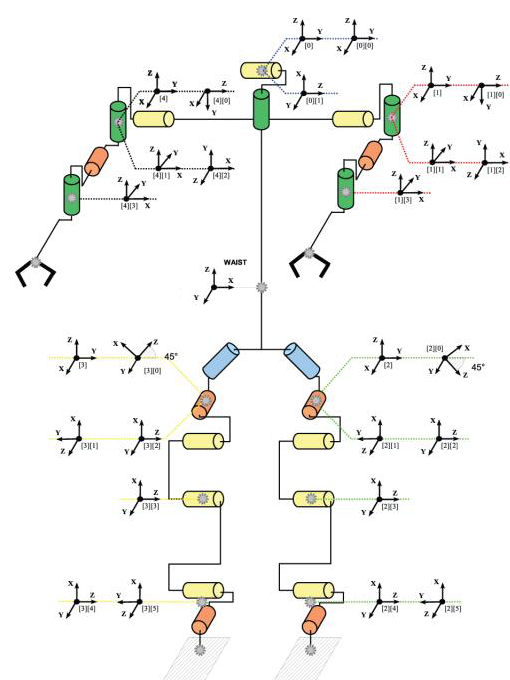
\includegraphics[scale=0.5]{figuras/nao_joints.png}
% \fonte{Retirada de \citeauthor{boedecker2008simspark}}~\label{fig:juntasNAO}
% \end{figure}

% Tabelas também devem ser referenciadas no texto e utilizadas como parte da explicação ou análise desenvolvida no capítulo. Deve ser referenciada como a Tabela~\ref{tab:tabelaTeste}. Observe que tanto figuras como tabelas devem ter suas legendas antes e a fonte indicada imediatamente após a figura ou tabela. Mesmo quando for criada pelo autor isto deve obrigatoriamente ser indicado segundo as normas da ABNT. As legendas devem ser auto-explicativas de forma que alguém que olhe a figura ou tabela e leia sua legenda consiga compreender tudo que vê sem necessidade de recorrer ao texto. O texto deve aprofundar e detalhar esta explicação, até repetindo algumas coisas que estão na legenda, mas principalmente vinculando à sequencia lógica do que está sendo exposto no texto.

% %%tabela
% \begin{table}[htb]
% \caption{Primeira tabela.}
% \begin{center}
% \begin{tabular}{|c|c|c|}
% \hline
% coluna 1 & coluna 2 & coluna 3 \\
% \hline
% valor 1,1 & valor 1,2 & valor 1,3 \\
% valor 2,1 & valor 2,2 & valor 2,3 \\
% \hline
% \end{tabular}
% \end{center}
% \fonte{Criada pelo autor.}
% \label{tab:tabelaTeste}
% \end{table}

%  Equações devem aparecer como parte natural do texto. Por exemplo energia pode ser definida como:

% %%equacao
% \begin{equation}
% E = m \times c^2,
% \label{eq1}
% \end{equation}

% \noindent onde $E$ é a energia, $m$ é a massa e $c$ é a velocidade da luz. Desta forma, apesar de numeradas, no local onde a equação aparece não será citada pelo número e sim como parte integrante do texto. Entretanto, às vezes é necessário fazer referência novamente à equação em um ponto posterior do texto (em outra seção ou mesmo em outro capítulo, ou num ponto mais distante dentro da mesma seção depois da ocorrência da mesma). Neste caso é usada a referência à Equação \eqref{eq1}.


% \section{Seção 2 do Capítulo 1 - Citações}
% Num texto científico é muito comum citar diversos autores lidos ou estudados. São feitas citações a livros, artigos científicos, etc. As normas ABNT regulamentam o formato das citações.

% São dois tipos de citações: diretas e indiretas. As citações diretas são feitas quando repete-se o texto citado igual ao original, com as mesmas palavras. Ou seja, a citação direta é uma cópia do trecho citado literalmente.

% Se a citação direta tiver menos que três linhas, deve ser feita entre aspas, assim: \foreignlanguage{english}{"This is one of the oldest leagues in RoboCupSoccer"}\cite{RoboCup}. Observe que se sua fonte for um texto em inglês ou outro idioma estrangeiro, deve se reproduzido no mesmo idioma original numa citação direta. Se você traduzir, isto vira uma citação indireta.

% Outro formato de citação direta é quando ela tem três ou mais linhas. Aí deve ser feita desta forma:
% \begin{citacao}[english]
% In the Humanoid League, autonomous robots with a human-like body plan and human-like senses play soccer against each other. Unlike humanoid robots outside the Humanoid League the task of perception and world modeling is not simplified by using non-human like range sensors. In addition to soccer competitions technical challenges take place. Dynamic walking, running, and kicking the ball while maintaining balance, visual perception of the ball, other players, and the field, self-localization, and team play are among the many research issues investigated in the Humanoid League. Several of the best autonomous humanoid robots in the world compete in the RoboCup Humanoid League\cite{RoboCup}.
% \end{citacao}


% Por fim, a forma mais comum de fazer uma citação é a indireta, quando você reproduz as ideias de um texto lido com as suas palavras. Ou seja, você não copia literalmente o texto de um autor, mas sim suas idéias, reescrevendo-as com suas palavras e de forma que faça sentido logicamente no seu texto. Isto vale inclusive para o caso em que reescrevemos em português as ideias de um texto lido em outro idioma. Neste caso a citação pode vir simplesmente logo ao final da ideia reproduzida, assim\cite{Alamdari2017}. Em alguns casos, você quer usar os autores como sujeito ou objeto de uma sentença. Por exemplo, quer dizer que \citeauthor{Xu2017} apresentaram alguma ideia ou ainda falar sobre algo que foi apresentado por \citeauthor{shafii2015learning}.


% Outra coisa comum é o uso de siglas (acrônimos). Ao utilizar uma sigla pela primeira vez, a mesma deve aparecer por extenso, assim: \gls{US}. Nas próximas ocorrências a sigla já aparecerá apenas como acrônimo, veja: \gls{US}. Qualquer nova sigla - como \gls{AA} - seguirá esta regra. Observe que siglas em inglês serão colocadas em itálico. Ao usar as siglas, as mesmas serão exibidas na Lista de siglas e abreviaturas entre os elementos pré-textuais.

%%%%%%%%%%%%%%%%%%%%%%%%%%%%%%%%%%%%%%%%%%%%%%%%%%%%%%%%%%%%%%%%%%%%%%%%%%%
%%%             DESCRICOES TEORICAS E FERRAMENTAS BASICAS               %%%
%%%%%%%%%%%%%%%%%%%%%%%%%%%%%%%%%%%%%%%%%%%%%%%%%%%%%%%%%%%%%%%%%%%%%%%%%%%

\setlength{\parskip}{0.3cm}

\chapter{Capítulo 2~-~Fundamentação Teórica}~\label{ch:fundamentacao}

\section{Biologia Molecular}
A Biologia Molecular é um ramo da biologia que lida e investigas os processos e mecanismos moleculares relacionados à estrutura, função e interações das biomoléculas presentes nos organismos vivos. Consiste em principalmente em estudar as interações entre os vários sistemas da célula, partindo da relação entre o \gls{dna}, \gls{rna} e a síntese de proteínas, e o modo como essas interações são reguladas.

É importante entender a estrutura do \gls{dna} vista na Figura~\ref{fig:estruturaDNA}, está é uma molécula em forma de dupla hélice que carrega a informação genética em organismos vivos. Ela é composta por duas cadeias polinucleotídicas complementares enroladas em torno de um eixo central. Cada cadeia é composta por uma sequência de nucleotídeos, que consistem em uma pentose (a desoxirribose), um grupo fosfato e uma base nitrogenada (adenina, timina, citosina ou guanina). A estrutura do \gls{dna} é mantida por pontes de hidrogênio entre as bases complementares, com a adenina pareando sempre com a timina e a citosina pareando sempre com a guanina.

%%figura
\begin{figure}[htb]
  \centering
  \caption{Estrutura do DNA.}
  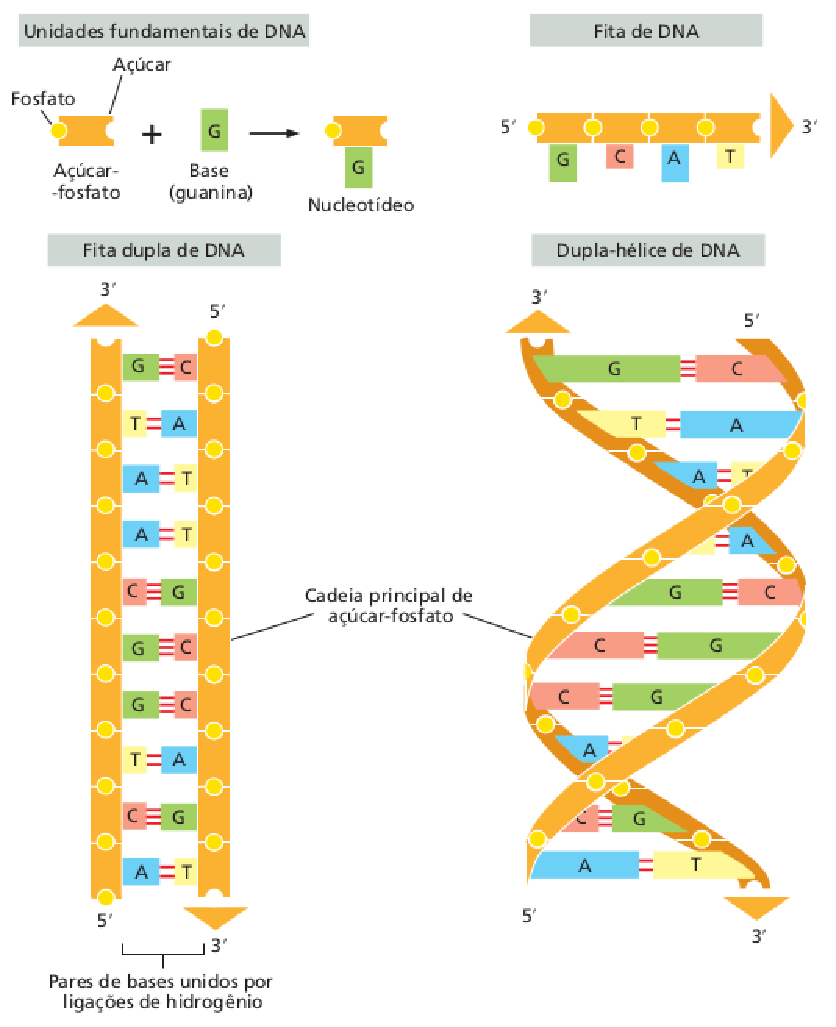
\includegraphics[scale=0.6]{figuras/estruturaDNA_02.pdf}
  \fonte{Retirada de \citeauthor{alberts_biologia_2017}}~\label{fig:estruturaDNA}
\end{figure}

As informações contidas no \gls{dna} é copiada em uma molécula de \gls{rna}, esse processo é conhecido como transcrição. A transcrição ocorre no núcleo das células e envolve a separação das duas fitas do \gls{dna} e o pareamento de nucleotídeos complementares para sintetizar uma molécula de \gls{mrna}. O \gls{mrna} é uma cópia do DNA que carrega a sequência de bases nitrogenadas correspondente a um gene específico.
Após isso, ocorre o processo de tradução onde a sequência de bases nitrogenadas do \gls{mrna} é utilizada para sintetizar proteínas. A tradução ocorre nos ribossomos, presentes no citoplasma celular. Durante a tradução, o \gls{mrna} é lido em grupos de três bases, chamados de códons. Os códons são sequências de três nucleotídeos consecutivos no RNA que correspondem a um aminoácido específico. Existem 64 códons possíveis, correspondentes a 20 aminoácidos diferentes como apresentado na Figura~\ref{fig:tabelaCodons}, além de sinais de início e parada da tradução. A tradução é o processo pelo qual a sequência de códons no RNA é utilizada para sintetizar proteínas. Durante a tradução, os códons são reconhecidos por moléculas de RNA transportador (tRNA) que trazem os aminoácidos correspondentes.
\begin{figure}[htb]
  \centering
  \caption{Tabela de Códons.}
  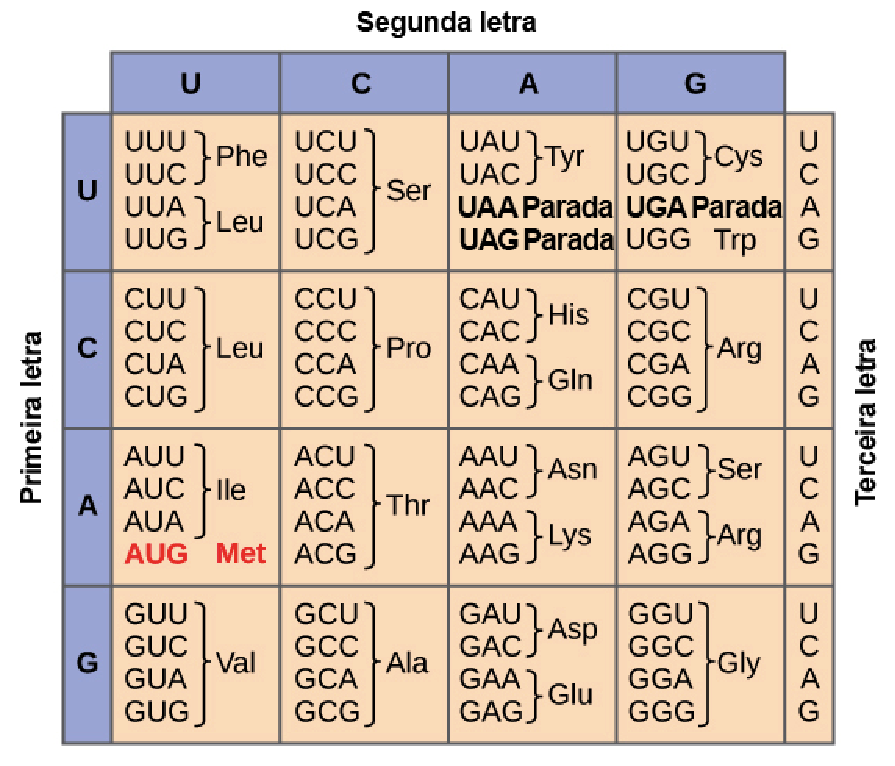
\includegraphics[scale=0.6]{figuras/tabelaCodons.pdf}
  \fonte{Adaptade de \citeauthor{openstax-genetic-code}}~\label{fig:tabelaCodons}
\end{figure}

A relação entre os códons, o DNA e o RNA é crucial para a síntese de proteínas e a expressão genética. O sequenciamento do DNA e a identificação dos códons correspondentes permitem a inferência das sequências de aminoácidos nas proteínas codificadas por um determinado gene.

Cada códon especifica um aminoácido distinto. Os aminoácidos são transportados para o ribossomo por moléculas de \gls{trna}, que possuem um anticódon complementar ao códon do \gls{mrna}. À medida que o ribossomo percorre o \gls{mrna}, os aminoácidos são ligados em uma sequência específica, formando uma cadeia polipeptídica que será dobrada e modificada para se tornar uma proteína funcional~\cite{alberts_biologia_2017}.

\section{Vírus}

Os vírus são agentes infecciosos que possuem uma estrutura viral que varia entre os seus diferentes tipos, mas que de modo geral é composta por uma cápsula proteica chamada capsídeo, que envolve o material genético viral, que pode ser \gls{dna} ou \gls{rna}. O capsídeo pode apresentar diferentes formas, como hélices, icosaedros ou formas complexas. Além do capsídeo, alguns vírus possuem uma camada lipídica chamada envelope viral, que é derivada da membrana da célula hospedeira e contém glicoproteínas virais que são importantes para a entrada do vírus nas células hospedeiras~\cite{david_virology_2022}.
O ciclo e vida viral é conjunto de etapas que um vírus passa para se reproduzir e infectar novas células. Esse ciclo pode variar entre diferentes tipos de vírus, mas geralmente envolve as seguintes etapas\cite{alberts_molecular_2002}:

\begin{enumerate}
  \item \textbf{Adsorção:} o vírus se liga especificamente a receptores na superfície da célula hospedeira.
  \item \textbf{Penetração:} o vírus é internalizado na célula hospedeira, liberando seu material genético.
  \item \textbf{Replicação e síntese de proteínas virais:} o material genético viral é transportado para os ribossomos da célula hospedeira, replicado e transcritas em moléculas de \gls{mrna}, que são utilizadas para a síntese de proteínas virais.
  \item \textbf{Montagem:} as proteínas virais se unem para formar novas partículas virais.
  \item \textbf{Liberação:} as novas partículas virais são liberadas da célula hospedeira, para a montagem de novos vírus e para a modificação do ambiente celular para garantir a sua replicação.
        % \item \textbf{Liberação:} as novas partículas virais são liberadas da célula hospedeira, podendo ocorrer por lise celular ou por brotamento
\end{enumerate}

\subsection{SARS-CoV-2}

O SARS-CoV-2 é um vírus da família Coronaviridae, que causa a doença chamada \gls{covid19}. Ele foi identificado pela primeira vez em dezembro de 2019 na cidade de Wuhan, na província de Hubei, na China, e desde então se espalhou para todo o mundo, resultando em uma pandemia global~\cite{zhu_novel_2020,wu_coronavirus_2020}.

O SARS-CoV-2 possui uma estrutura viral apresentada na Figura~\ref{fig:estruturaCoronavirus}, característica dos coronavírus. Ele é composto por uma partícula viral esférica, com um envelope lipídico que envolve seu material genético. A estrutura do vírus inclui proteínas de espículas na sua superfície, conhecidas como proteína spike (S), que são responsáveis pela ligação do vírus às células hospedeiras. Além disso, o SARS-CoV-2 possui proteínas de membrana (M), envelope (E) e nucleocapsídeo (N), que desempenham papéis importantes na estrutura e na replicação viral.

\begin{figure}[htb]
  \centering
  \caption{Estrutura do coronavírus.}
  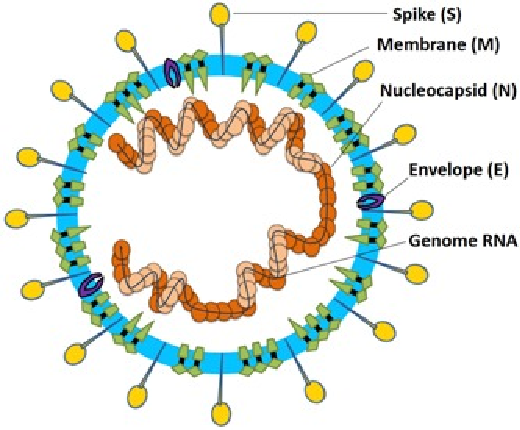
\includegraphics[scale=0.8]{figuras/estruturaSarsCov2.pdf}
  \fonte{Retirada de \citeauthor{li_coronavirus_2020}}~\label{fig:estruturaCoronavirus}
\end{figure}

\section{Filogenia}

A filogenia é uma disciplina da biologia que estuda as relações evolutivas entre organismos, buscando reconstruir a história evolutiva e a ancestralidade comum. A filogenética molecular é uma abordagem utilizada para inferir a filogenia com base em informações moleculares, como sequências de \gls{dna}, \gls{rna} e proteínas\cite{felsenstein_inferring_2004}.

A construção de árvores filogenéticas é um aspecto fundamental da filogenética molecular. Existem vários métodos utilizados para construir árvores filogenéticas, que podem ser classificados em dois grupos principais: métodos baseados em distância e métodos baseados em caracteres.
Os métodos baseados em distância medem a similaridade ou a dissimilaridade entre sequências moleculares e constroem árvores filogenéticas com base nessas medidas. Alguns exemplos de métodos baseados em distância incluem o método de Neighbor Joining (NJ) e o método de Mínima Evolução (ME).
Por outro lado, os métodos baseados em caracteres analisam as mudanças nos caracteres moleculares ao longo do tempo para inferir as relações filogenéticas. Exemplos de métodos baseados em caracteres são o método de Máxima Parcimônia (MP) e o método de Inferência Bayesiana\cite{swofford_phylogenetic_1996}.

% \section{Bioinformática}

% Alinhamento de Sequências, Análise de Genomas Virais, Análise de Expressão Gênica, Ferramentas de Bioinformática

% \section{Machine Learning}

% Escrever sobre

\section{Trabalhos Correlatos}

% Para iniciar, vamos testar novamente o uso de siglas: \gls{AA}. Observe que mesmo ao iniciar outro capítulo, a sigla não precisa ser definida novamente por extenso, pois já foi definida no capítulo anterior, além de estar definida na lista de siglas e abreviaturas.

% A partir do capítulo~\ref{ch:fundamentacao} começa-se a apresentar a fundamentação teórica. Atenção ! Fundamentação teórica não é o mesmo que trabalhos relacionados ou estado da arte. Fundamentação teórica são conceitos teóricos - alguns mesmo antigos ou clássicos - que precisam ser compreendidos para entender a solução apresentada para o problema investigado.

% Não há um modelo de divisão de capítulos. Alguns autores criam um único capítulo chamado `Fundamentação Teórica' e nele colocam todos os conteúdos divididos em seções, subseções, etc. Outros preferem criar capítulos diferentes para temas diferentes da fundamentação teórica. Enfim, não há uma regra rígida para isto. Deve ser definido em consenso com o orientador. O importante é ter bom senso para não criar vários capítulos minúsculos com 1 página ou menos. Se o que tem para falar de um tema é tão pouco, talvez valha à pena ter um único capítulo de fundamentação teórica com várias seções falando dos diversos temas que compõem sua fundamentação. Mas se cada tema tem muito a ser falado, pode ficar melhor dividi-los em capítulos diferentes.

% Quanto a Trabalhos Relacionados ou Estado da Arte eles são as publicações recentes de pessoas que tentaram resolver o mesmo problema ou um problema similar. São o resultado da revisão sistemática de literatura feita no início do processo de TCC. Alguns autores optam por fazer a análise destes trabalhos dentro do capítulo de introdução. Outros optam por criar um capítulo denominado "Estado da Arte" ou "Revisão de Literatura" ou "Trabalhos Relacionados" e fazer esta análise lá. A decisão mais uma vez fica a critério de cada autor e deve ser tomada em consenso com o orientador. Se os Trabalhos Relacionados estiverem na introdução, certamente irá gerar uma introdução mais longa. Mas não há problema ou impedimento quanto a isto.

% Uma vantagem de colocar na introdução é que logo no início da monografia já ficam claras as lacunas do estado da arte que seu trabalho buscará preencher. Quando feito num capítulo à parte isto só aparece depois, mas gera o benefício de não deixar a introdução tão extensa e por vezes cansativa para o leitor. Então é uma questão de decisão do autor e do orientador.

% Quando colocado num capítulo à parte costuma vir antes dos capítulos de fundamentação teórica.
%%%%%%%%%%%%%%%%%%%%%%%%%%%%%%%%%%%%%%%%%%%%%%%%%%%%%%%%%%%%%%%%%%%%%%%%%%%
%%%                         O MODELO                                    %%%
%%%%%%%%%%%%%%%%%%%%%%%%%%%%%%%%%%%%%%%%%%%%%%%%%%%%%%%%%%%%%%%%%%%%%%%%%%%

\chapter{Descrição do Projeto}

% objetivos, ponto de partida, produtos e resultados esperados, tecnologias a serem usadas.
% + estrutura da solução nas fases de treinamento e aplicação

% ### METODOLOGIA ###

% ### Falar das seguintes ferramentas:
%   - DSR
%   - Trello
%   - Github

A seguir, serão apresentadas a metodologia e os softwares utilizados neste estudo, bem como as etapas detalhadas de sua implementação.

% Metodologia
\section{Metodologia}~\label{sec:metodologia}
Um ponto importante para a obtenção dos objetivos deste trabalho está relacionada a definição da metodologia que servirá como alicerce. Com a proposta de desenvolver e validar um método de análise da evolução molecular de vírus com base no uso de códons, a metodologia escolhida para isso é o \gls{dsr}. Essa metodologia, proporciona um framework teórico e prático para a criação de artefatos inovadores, como métodos, modelos ou frameworks, visando resolver problemas específicos~\cite{peffers_dsr_2007}. Neste projeto, a ferramenta de análise de genes virais baseada em códons é o artefato que será desenvolvido e avaliado. Além disso, o \gls{dsr} enfatiza a validação e a avaliação da utilidade e eficácia do artefato em relação aos seus objetivos práticos. No caso deste projeto, a validação será realizada através da comparação dos resultados obtidos com a ferramenta proposta em relação às técnicas clássicas filogenéticas, que são amplamente utilizadas para a análise de genes virais. Essa comparação permitirá avaliar a eficácia e o valor agregado da abordagem baseada em códons.

Para a obtenção de sucesso ao utilizar o \gls{dsr} os seguintes passos serão seguidos:
\begin{enumerate}
  \item Identificação do problema e definição dos objetivos.
  \item Desenvolvimento dos artefatos.
  \item Avaliação do artefato.
  \item Apresentar contribuições científicas.
\end{enumerate}

Também será utilizada analises quantitativas, ou seja, medidas estatísticas para mensurar e comparar os resultados obtidos.\\
A pesquisa quantitativa só tem sentido quando há um problema muito bem definido e há informação e teoria a respeito do objeto de conhecimento, entendido aqui como o foco da pesquisa e/ou aquilo que se quer estudar. Esclarecendo mais, só se faz pesquisa de natureza quantitativa quando se conhece as qualidades e se tem controle do que se vai pesquisar.~\cite{da_silva_pesquisa_2014}

\section{Materiais e Métodos}
Nesta sessão, será apresentada as ferramentas utilizadas para a construção e desenvolvimento de todo o trabalho.

O Python é uma linguagem de programação de alto nível, interpretada, iterativa e de código aberto. Foi criada por Guido van Rossum e lançada em 1991. A linguagem é conhecida por ter uma sintaxe simples, tornando-a popular para o desenvolvimento de software, automação, análise de dados, aprendizado de máquina entre outras aplicações. A mesma apresenta suporte a vários paradigmas de programação, como a orientada a objetos, imperativa, procedural e funcional. Além disso, o Python é portátil, podendo ser executado em diversos sistemas operacionais como Linux, Mac e Windows.~\cite{python-reference}

Para a construção dos pipelines do projeto, utilizamos Python em conjunto com o Jupyter Notebook. O Jupyter Notebook é uma aplicação de código aberto que permite criar documentos interativos que integram código, texto narrativo e visualizações. É uma ferramenta amplamente adotada por cientistas de dados, pesquisadores e desenvolvedores para explorar dados, prototipar código, documentar projetos e facilitar a colaboração. Além disso, o Jupyter Notebook oferece suporte a diversas linguagens de programação, incluindo Python~\cite{jupyter-notebook}.

O python possui uma gama de bibliotecas que facilitam a implementação de soluções complexas. A seguir serão apresentadas a bibliotecas utilizadas:

\begin{itemize}
  \item \textbf{Biopython}: Coleção de bibliotecas e ferramentas em Python, disponíveis gratuitamente para biologia molecular computacional. Ele fornece uma ampla gama de funcionalidades, desde a leitura e análise de arquivos de sequência biológica até a execução de algoritmos sofisticados de bioinformática. Desenvolvida e mantida pelo Projeto Biopython, que é uma associação internacional de desenvolvedores de ferramentas python.~\cite{biopython}
  \item \textbf{Selenium}: Biblioteca de código aberto que fornece uma interface programática para automatizar interações com navegadores da web. É amplamente utilizado por desenvolvedores e testadores de software para realizar testes automatizados, raspagem de dados na web e outras tarefas que envolvem interações com páginas da web. O Selenium para Python permite a automação de ações como clicar em botões, preencher formulários, navegar em sites e extrair informações da web, tornando-o uma ferramenta valiosa para desenvolvimento e automação de tarefas na web.~\cite{selenium-python}
\end{itemize}

% Lista de Tecnologias/Ferramentas utilizadas:
% Python 3 ok
% Selenium ok
% Biopython ok
% Shell (verificar necessidade)
% Jupyter Notebook ok
% Minimap2
% GoFasta
% virtualEnv
% BV_BRC - O \gls{bvbrc}, é um centro de recursos de bioinformática dedicado ao estudo e análise de bactérias e vírus. O site também disponibiliza uma uma coleção abrangente de banco de dados, incluindo sequências genômicas, anotações funcionais, informações de expressão gênica e estruturas tridimensionais. O acesso aos bancos de dados é dado por meio de uma interface amigável, onde é possível realizar pesquisas avançadas.

% AGUA (verificar e apresentar os sub-softwares utilizados, ex.: CLOPE)

\section{Plano de Implementação}
% Lista de Tecnologias/Ferramentas utilizadas:
% Python 3
% Selenium
% Biopython
% Shell (verificar necessidade)
% Jupyter Notebook
% Minimap2
% GoFasta
% virtualEnv
% AGUA (verificar e apresentar os sub-softwares utilizados, ex.: CLOPE)

Durante o desenvolvimento do projeto foi necessário dividir o projeto em fases com base nas atividades que deveriam ser realizadas de forma a atender todos os passos descritos na seção~\ref{sec:metodologia}. As principais fases identificadas foram: Montagem e preparação do dataset a ser utilizado pelo modelo; Desenvolvimento completo do modelo, com todos as definições, implementações, testes e correções necessárias; e a análise comparativa que será realizada com um outro método existente e já tradicional. Esses pontos são apresentados de forma minuciosa a seguir.

\subsection{Montagem e Preparação do Dataset}
% Verificar como descrever os dois conjuntos de pipelines montados. Pip 01 (Descartado) - Pip 02 (Atual)
Para realizar o treinamento do modelo a ser construído, eram necessárias sequências únicas e alinhadas do gene Spike. Em vista disso, é importante salientar que o site \gls{bvbrc} disponibiliza sequências genômicas, e sendo assim, foi preciso construir um pipeline para, após o download das sequências, transformar as mesmas para a criação de um dataset com as sequências que atendessem os requisitos esperados.

Inicialmente, foi realizada uma analise do \gls{bvbrc}, para entende a sua estrutura e verificar também se era possível realizar o download de todas as sequências queridas de forma manual. Foi verificado que o site possuía uma área de seleção de filtros, e foi definido que só seriam selecionadas sequências completas no campo \textit{Genome Status} e no campo \textit{Lineage}, onde é possível filtrar as sequências pelo seu tipo \textit{Pango} e também verificar a quantidade, só os que tivessem mais de 50 sequências do mesmo tipo.

Após a análise, foi constatado que realizar o download manualmente era infactível, e que seria preciso automatizar esse processo de iteração com a página, como vistos na Figura~\ref{fig:pipelineBvbrc}. Isto posto, foi realizado uma sequência de passos conhecidos como \textit{Web Scrapping} utilizado o Python juntamente com o Selenium, apresentados em seguida:

\begin{figure}[htb]
  \centering
  \caption{Pipeline de Download das Sequências Genômicas.}
  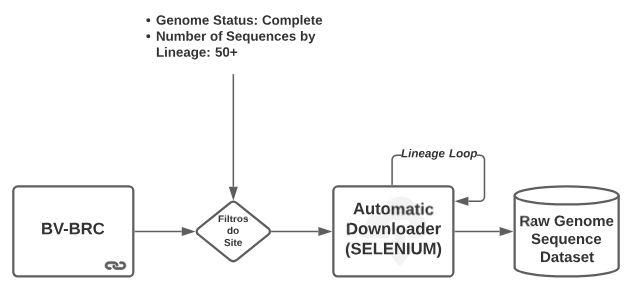
\includegraphics[scale=0.6]{figuras/pipelines/bvbrc.png}
  \fonte{O Autor}~\label{fig:pipelineBvbrc}
\end{figure}

\begin{enumerate}
  \item Criar uma lista com todos as linhagens disponíveis e a quantidade de sequências de cada.
  \item Desenvolver script Python para remover as linhagens com menos de 50 sequências da lista.
  \item Desenvolver script Python para gerar uma url personalizada do \gls{bvbrc}, já com os filtros, para cada linhagem.
  \item Desenvolver script Python juntamente com o Selenium para abrir as urls de forma automática e realizar o download das sequências.
\end{enumerate}

Ao final do processo de montagem do dataset, realizado no dia 02 junho de 2023, com sequências genômicas completas, foi gerado um diretório raiz (dataset), e dentro deste, um diretório para cada linhagem (\textit{Lineage} L¹, \textit{Lineage} L², \dots, \textit{Lineage} $L^{n}$), contendo um arquivo nomeado \textnormal{BVBRC\_genome\_sequence.fasta}, como apresentado na figura~\ref{fig:datasetGenomas}.

\begin{figure}[htb]
  \centering
  \caption{Dataset de sequências genômicas.}
  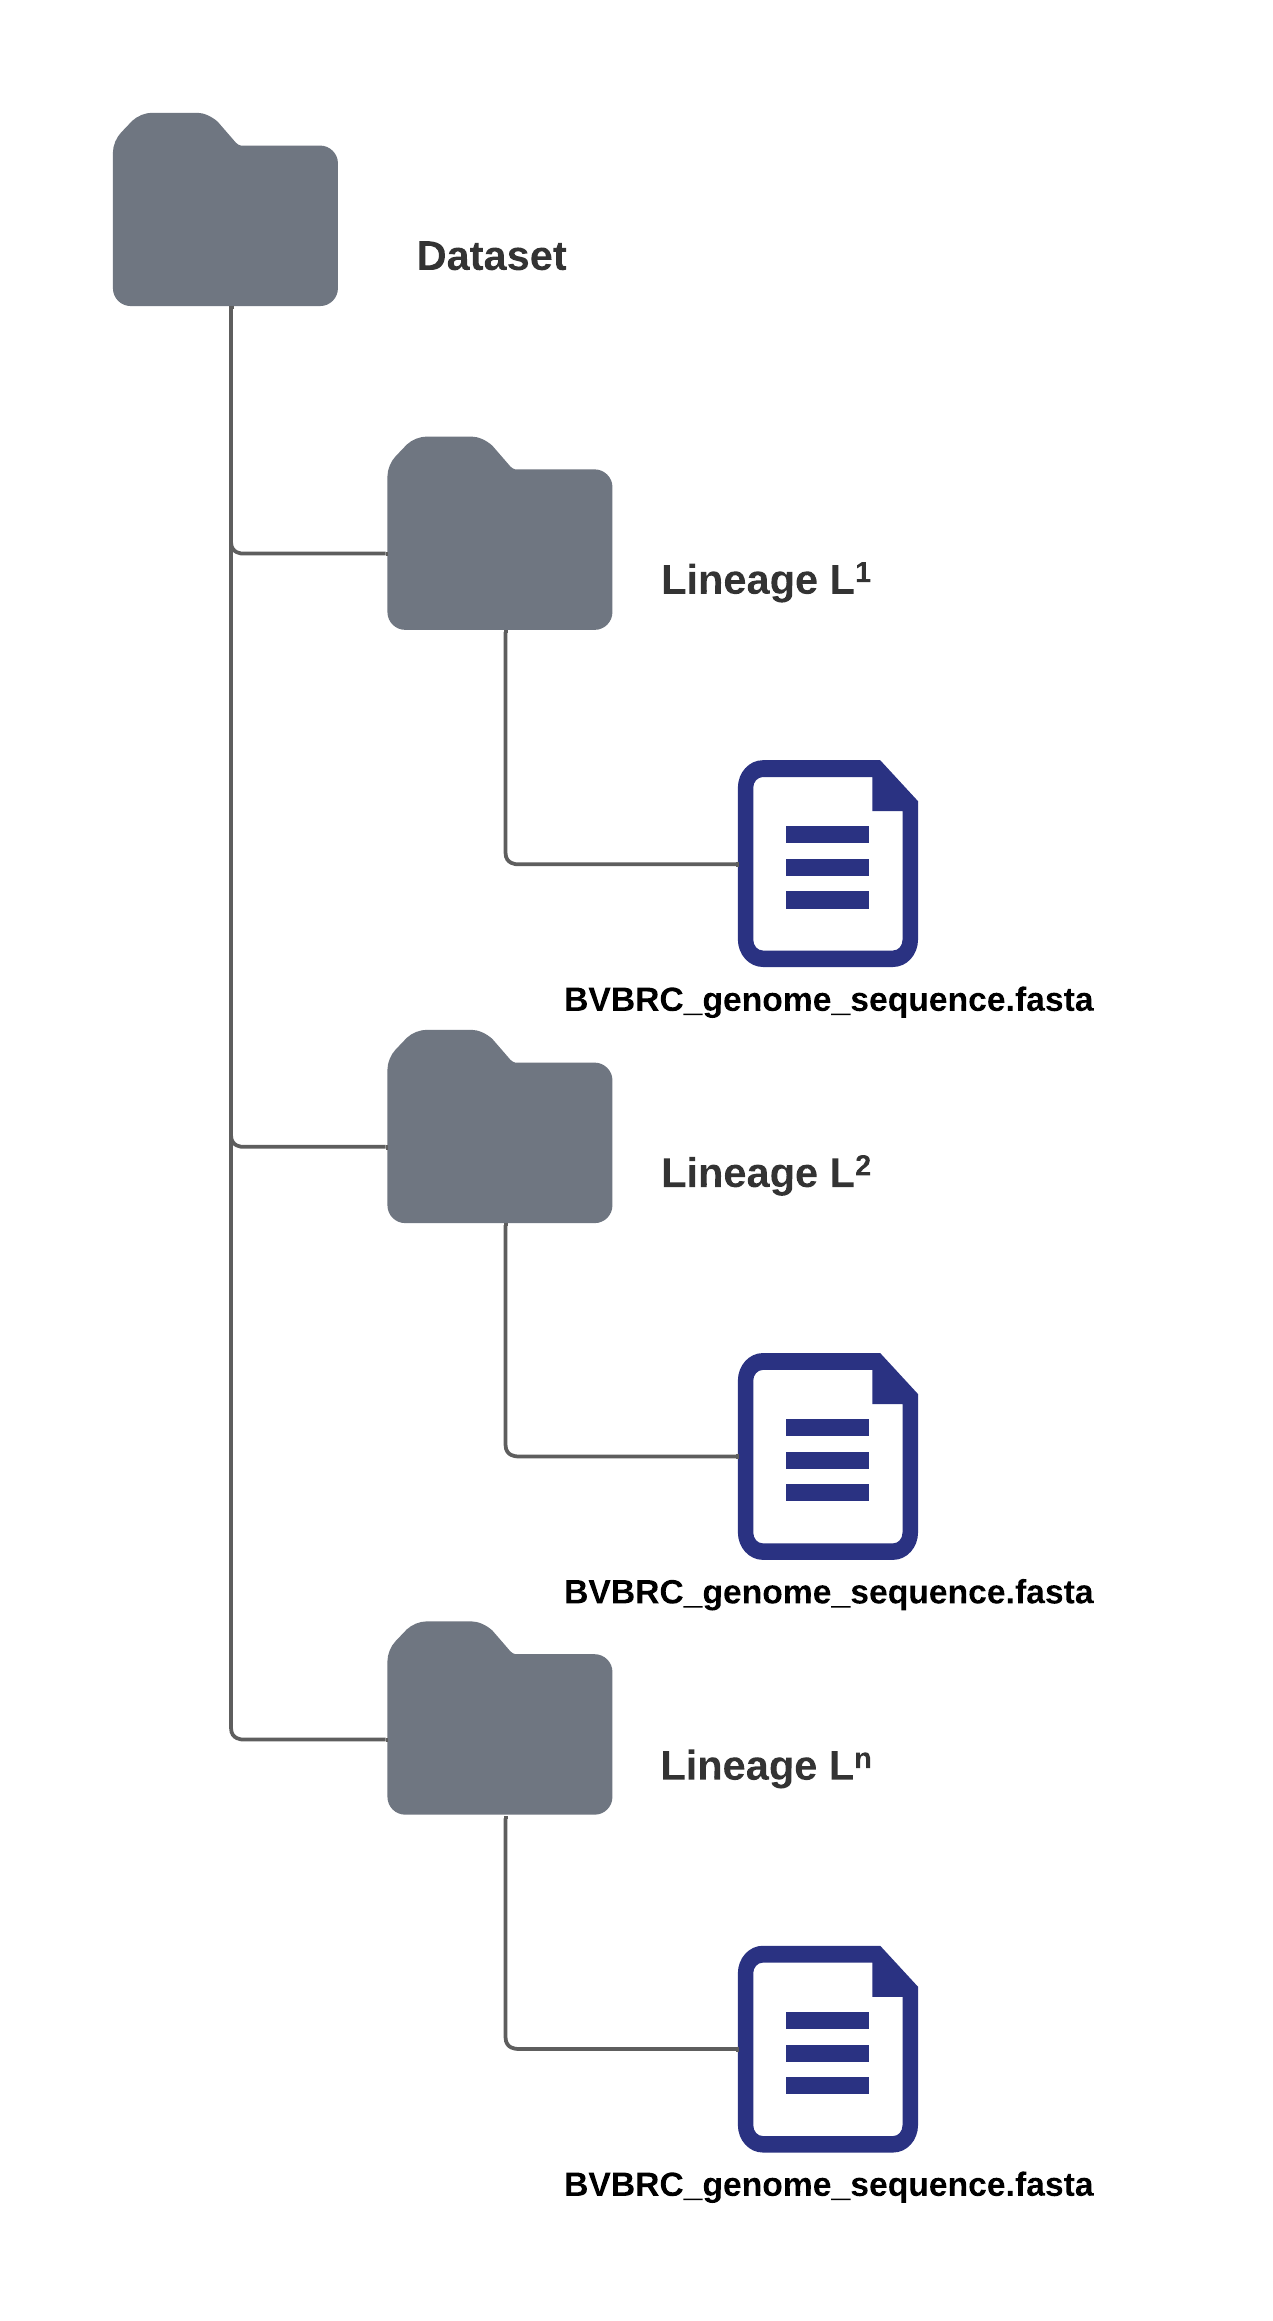
\includegraphics[scale=0.5]{figuras/dataset_principal.png}
  \fonte{O Autor}~\label{fig:datasetGenomas}
\end{figure}

Ao finalizar o processo de download, o dataset completo ficou com as seguintes informações apresentadas na tabela~\ref{tab:datasetGenomas}.

%%tabela
\begin{table}[htb]
  \caption{Informações do dataset de sequências genômicas.}
  \begin{center}
    \begin{tabular}{|c|c|}
      \hline
      Campo                              & Valor     \\
      \hline
      Quantidade de Linhagens            & 1086      \\
      Quantidade de Sequências Genômicas & 1.494.650 \\
      Tamanho em \gls{gigabyte}          & 47.5      \\
      \hline
    \end{tabular}
  \end{center}
  \fonte{Criada pelo autor.}\label{tab:datasetGenomas}
\end{table}

A seguir, era necessário construir um dataset de sequências do gene Spike a partir do existente. Para isso, com o objetivo de diminuir o tempo de execução dos pipelines durante o desenvolvimento, foi construído também, um dataset de testes, apresentado na tabela~\ref{tab:datasetGenomasTeste}, que serviria como base para execução das atividades, e após as verificações, seria realizado o processo com o dataset completo. No dataset de testes, foram escolhidas 5 (cinco) linhagens que são amplamente conhecidas (gamma, delta, alpha, beta e omicron), o que tornaria mais preciso o processo de validação futuramente.

\begin{table}[htb]
  \caption{Informações do dataset de teste de sequências genômicas.}
  \begin{center}
    \begin{tabular}{|c|c|c|c|}
      \hline
      Pango     & \gls{who} & Quantidade de Sequências & Tamanho em \gls{megabyte} \\
      \hline
      B.1.1.7   & Alpha     & 9982                     & 307                       \\
      B.1.1.529 & Omicron   & 3694                     & 112.7                     \\
      B.1.351   & Beta      & 5256                     & 160.6                     \\
      B.1.617.2 & Delta     & 9996                     & 305.3                     \\
      P.1       & Gamma     & 10000                    & 305.9                     \\
      \hline
      Total     &           & 38928                    & 1191,5                    \\
      \hline
    \end{tabular}
  \end{center}
  \fonte{Criada pelo autor.}\label{tab:datasetGenomasTeste}
\end{table}

Depois, foi verificado a existência de sequências genômicas idênticas, melhor dizendo, sequências com exatamente a mesma quantidade e ordem dos nucleotídeos. Por isso, foi necessário desenvolver um pipeline que filtrasse as sequências repetidas, e mantivesse apenas uma, como exibido na figura~\ref{fig:pipelineGenomicasDuplicadas}, gerando assim um novo dataset de sequências genômicas únicas.

\begin{figure}[htb]
  \centering
  \caption{Pipeline de Filtragem de Sequências Genômicas Duplicadas.}
  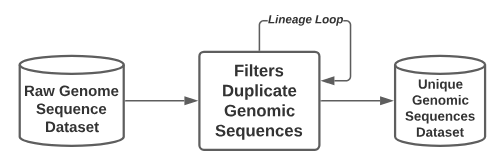
\includegraphics[scale=0.6]{figuras/pipelines/seqs_genomicas_duplicadas.png}
  \fonte{O Autor}~\label{fig:pipelineGenomicasDuplicadas}
\end{figure}

Com o dataset de sequências únicas montado, foi decidido os passos a seguir, que seriam executados com o papel de atingir o objetivo de obter o dataset de sequências gênicas únicas e alinhadas. Primeiro, como visto na figura~\ref{fig:pipelinesDescontinuados}, foi realizado o processo de extração do gene Spike, utilizando uma sequência de referência do gene obtida do dataset da \gls{ncbi}\footnote{Url para download: \url{https://www.ncbi.nlm.nih.gov/nuccore/NC_045512.2?report=genbank&from=21563&to=25384}}, juntamente com o software Blast, para encontrar e extrair o gene Spike de cada uma das sequências genômicas de todo o dataset. Após isso, com o dataset de sequências genicas já montado, era necessário realizar o processo de alinhamento das sequências. Foram verificada duas formas de realizar esse procedimento utilizando o software Clustalo Omega, uma passando uma sequência por vez (\textit{sequence by sequence}) com a sequência do Spike de referência e outra passando todas as sequências com a referência (\textit{multiple sequence}). Mesmo com o dataset de teste, que possuía um tamanho e quantidade de sequências muito inferior ao principal, o processo de alinhamento apresentou uma demora excessiva (até 2 dias) para finalizar. Em decorrência disso, o processo foi descontinuado, e um novo foi repensado e reconstruído e será apresentado a seguir.

\begin{figure}[htb]
  \centering
  \caption{Pipelines descontinuado.}
  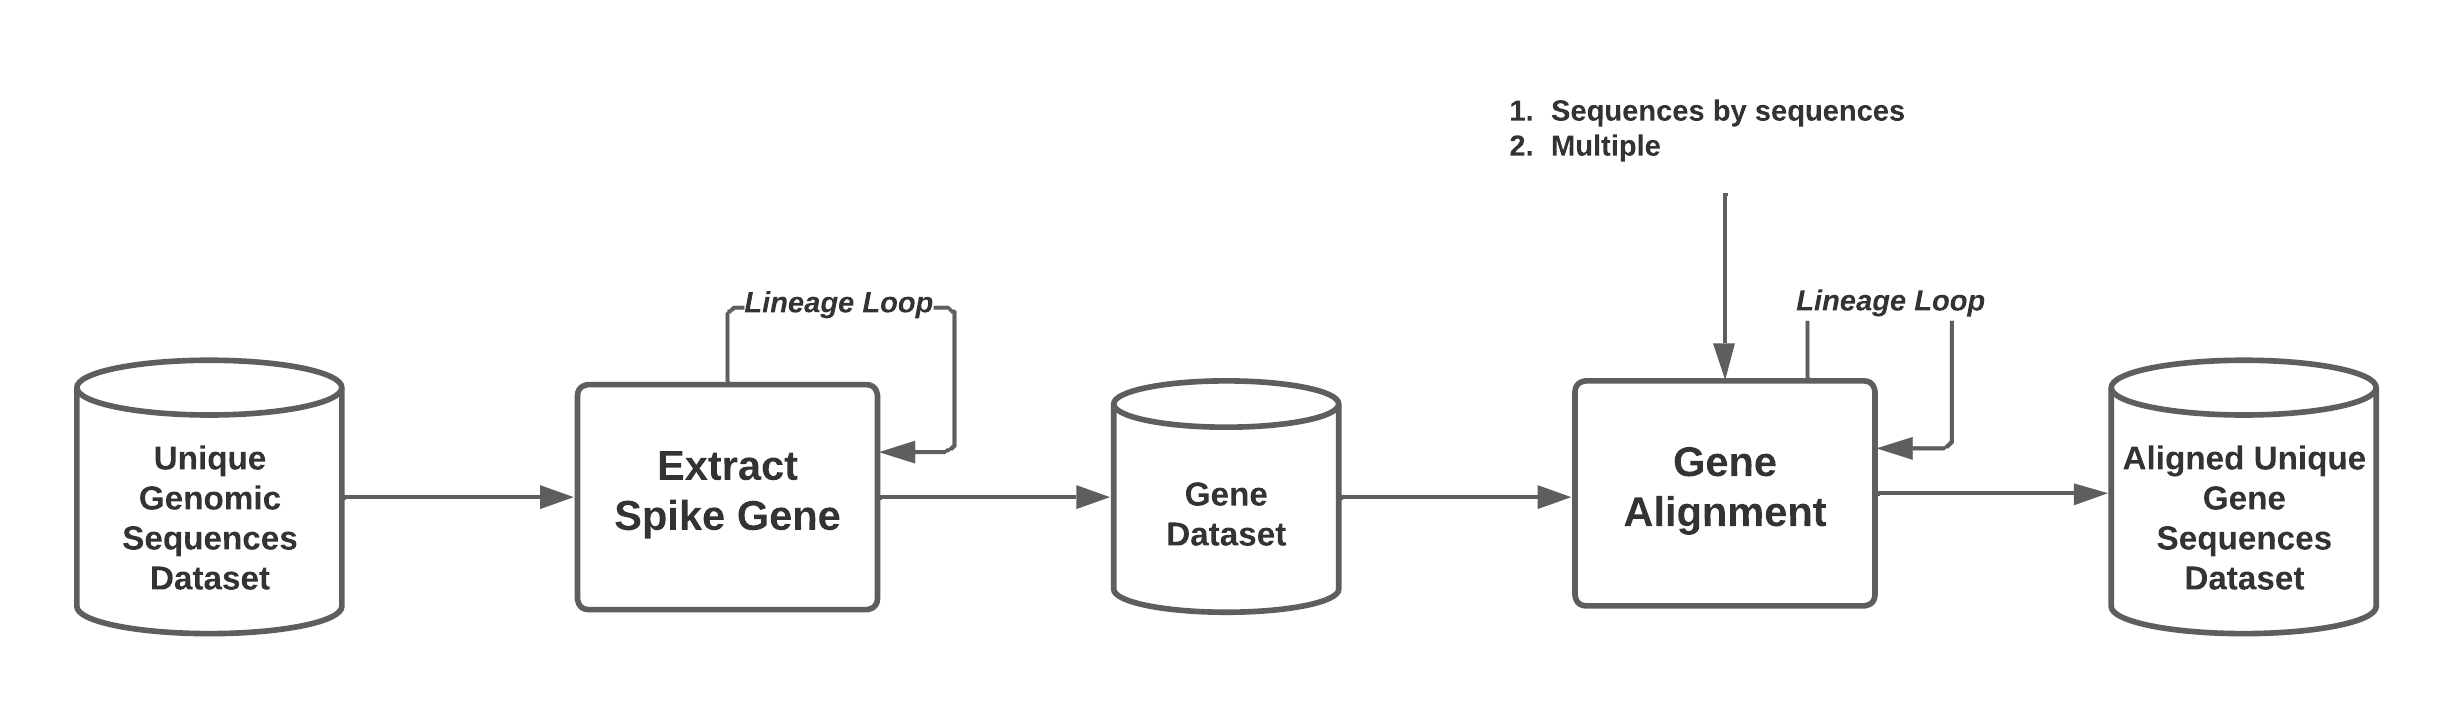
\includegraphics[scale=0.45]{figuras/pipelines/pipelines_descontinuado.png}
  \fonte{O Autor}~\label{fig:pipelinesDescontinuados}
\end{figure}

% FAZER
% Como escrever essa parte: Após análise; Após orientação do coorientador...
% Reescrever a lista abaixo de forma descritiva
% Substituir onde estiver citando 'modelo desenvolvido' pelo nome AGUA

Após a análise com os orientadores, o processo, que continuou a partir das sequências genômicas únicas, foi feito da seguinte maneira:

\begin{itemize}
  \item Alinhamento das sequências genômicas.
  \item Extração do gene spike.
  \item Filtragem das sequências genicas repetidas.
  \item Filtragem das sequências genicas de má qualidade.
\end{itemize}

Ao final do processo, foi gerado um dataset contendo sequências gênicas únicas para as variantes alpha, beta, delta, gamma e omicron.
A partir deste dataset, foi elaborado 2 (dois) arquivos, conforme a figura\ref{fig:inputAgua} apresenta, que serviria de entrada, tanto para o modelo desenvolvido como para a geração de árvores filogenéticas utilizando o modelo convencional, a fim de se realizar análises futuras. Um arquivo compreendia a mescla de sequências genicas de cada uma das linhagem, e um arquivo de anotações que serviria como base no treinamento, contendo o cabeçalho da sequência, na mesma ordem em que estava no arquivo mesclado, juntamente com a linhagem da sequência.

\begin{figure}[htb]
  \centering
  \caption{Arquivos de entrada do modelo.}
  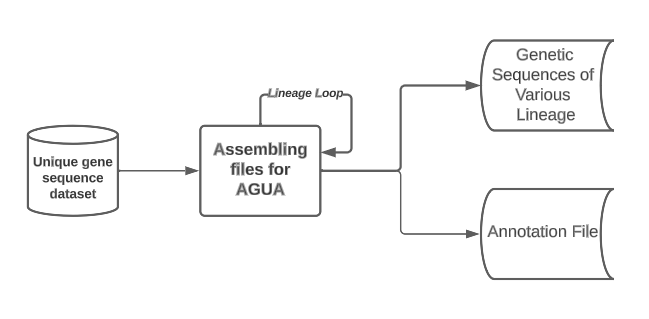
\includegraphics[scale=0.45]{figuras/pipelines/input_AGUA.png}
  \fonte{O Autor}~\label{fig:inputAgua}
\end{figure}

%   % Verificar se é melhor descrever o processo ou listar os itens como está atualmente
%   \item \textbf{Montagem e Preparação do Dataset:}  Abaixo, está apresentado o passo a passo que foi realizado nesta etapa:
%         \begin{itemize}
%           \item Analise do site \gls{bvbrc}.
%           \item Desenvolvimento de um script Python juntamente com o Selenium, para o download automático das sequências genomicas no \gls{bvbrc}.
%           \item Filtragem das sequências genômicas duplicadas, ou seja, que contenham exatamente, a mesma sequência de nucleotídeos, mantendo apenas 1(uma) das repetidas e construindo um dataset de sequências genomicas únicas. (Filtro 01)
%           \item Alinhamento das sequências genomicas utilizando o Minimap2.
%           \item Implementado procedimento de extração do gene de interesse (Spike), com base em uma sequência Spike de referência, das sequências únicas.
%           \item Filtragem das sequências genicas duplicadas, ou seja, que contenham exatamente, a mesma sequência de nucleotídeos, mantendo apenas 1(uma) das repetidas e construindo um dataset de sequências genicas únicas. (Filtro 02)
%           \item Filtragem das sequências genicas de má qualidade. Foram removidas as sequências que possuiam mais de 30 N's consecultivos ou que ficaram com a quantidade de nucleotídeos discrepantes em relação a referência genica. (Filtro 03)
%           \item Criar arquivo de treinamento com linhagens diferentes e um arquivo de anotação. % Descrever melhor os arquivos
%         \end{itemize}

\subsection{AGUA}
O modelo proposto foi nomeado como \gls{agua}. A seguir o mesmo será apresentado, desde a sua concepção, implementação e testes.

% FAZER
% Escrever uma descrição melhor do desenvolvimento do modelo
\begin{itemize}
  \item Levantamento dos requisitos.
  \item Definir a arquitetura e a abordagem do modelo de classificação baseado em códons.
  \item Implementar o modelo utilizando uma biblioteca ou framework adequado.
  \item Desenvolver algoritmo para traduzir as sequências de \gls{dna} em sequências de códons.
  \item Realizar treinamento do modelo utilizando os dados preparados.
  \item Avaliar o desempenho do modelo utilizando métricas apropriadas.
        % \item \item Avaliar o desempenho do modelo utilizando métricas apropriadas, como acurácia, precisão e recall.
  \item Identificar possíveis problemas e realizar ajustes no modelo.
        % \item Identificar possíveis problemas de overfitting ou underfitting e realizar ajustes no modelo, como ajuste de hiperparâmetros ou utilização de técnicas de regularização.
\end{itemize}

\subsection{Análise comparativa entre o método proposto e outro método existente}

% FAZER
% Descrever as ferramentas utilizadas aqui, quando falar do processo filogenético tradicional...

Será realizada uma analise com um conjunto de dados, onde será realizado analises estatísticas para verificação de melhorias, ou não, do novo método proposto analisando os seguintes aspectos:
\begin{itemize}
  \item Comparação dos métodos de agrupamento adotados, avaliando sua eficácia na formação de clusters e na identificação de padrões ou similaridades nas sequências.
  \item Avaliação do custo computacional (tempo de execução e recursos requeridos) para a classificação das sequências em cada método.
  \item Comparação da eficiência computacional entre os métodos, considerando a escalabilidade e o desempenho em grandes volumes de dados.
\end{itemize}

% \section{Plano de Testes e Validação}

% \section{Resultados Obtidos}
\chapter{Considerações finais}

Nesta fase inicial do projeto, foi realizada com sucesso a montagem do dataset de genes virais a serem estudados. Através do uso de scripts e procedimentos adequados, foram baixadas sequências classificadas de genoma completo do vírus de uma base de dados pública, como o \gls{bvbrc}, e em seguida, filtradas para manter apenas as sequências únicas. Além disso, o gene de interesse foi extraído utilizando a técnica de blast.

A montagem do dataset é uma etapa crucial para o desenvolvimento da ferramenta de análise de genes virais baseada em códons. Ao obter uma base de dados representativa e de qualidade, garantimos que a análise subsequente seja feita em um conjunto abrangente de sequências relevantes.

No entanto, é importante ressaltar que essa é apenas uma etapa inicial do projeto e que há muito trabalho a ser feito nas próximas fases. A análise comparativa entre o método proposto e outro método existente, bem como a implementação do modelo de classificação e as etapas subsequentes do processo, ainda estão por vir.

Com base na conclusão desta etapa, temos uma base sólida de dados que nos permitirá avançar no desenvolvimento do projeto. O próximo passo será a implementação do modelo de análise de genes virais baseado em codons e a realização das etapas subsequentes, como o alinhamento, a tradução e a extração de códigos únicos para a classificação e agrupamento das sequências.

A montagem bem-sucedida do dataset é um marco importante para o progresso do projeto, fornecendo a base necessária para a etapa seguinte. Com um dataset representativo e de qualidade, podemos agora prosseguir para a implementação do modelo e a análise comparativa com outras abordagens existentes.

% Neste capítulo são apresentadas duas coisas: Conclusões e Trabalhos Futuros. Aqui devem ser apresentadas a que conclusões se pode chegar a partir dos resultados apresentados e analisados no capítulo anterior. Um erro grave e recorrente é usar este capítulo para REPETIR coisas que já foram ditas. Não precisa dizer aqui o que você fez, isto já foi dito no capítulo de desenvolvimento projeto. Não precisa aqui repetir todos os resultados, isto já foi apresentado antes também. Você pode referenciar os seus principais resultados para fundamentar suas conclusões.

% Outro ponto é ter cuidado com o que se conclui. Pergunte sempre se realmente seus resultados permitem concluir o que você escreveu que está concluindo. Neste ponto das conclusões é onde você deve deixar evidente qual a principal contribuição de seu trabalho e quais as contribuições complementares/secundárias. Esta é uma pergunta que todo membro de banca examinadora tem na cabeça, então se já tiver claro aqui na conclusão é melhor.

% Finalmente sugira trabalhos futuros que façam sentido a partir dos seus resultados. Trabalhos estes que poderão ser desenvolvidos por você mesmo ou outras pessoas. São uma espécie de continuidade deste trabalho.

% Depois da conclusão virão os elementos pós-textuais: Glossários, Referências Bibliográficas, Apêndices e Anexos. Apenas as Referências Bibliográficas são obrigatórias e devem estar de acordo com as normas da ABNT.

%  O Apêndice é algum conteúdo complementar não obrigatório gerado pelo próprio autor. Por exemplo, um manual de uso de um sistema, diagramas de classe de um sistema, código-fonte completo ou parcial de um sistema. Enfim, coisas que não são necessárias para entender a solução e os resultados mas que podem ser úteis para alguém que queira se aprofundar mais. Como dito, é opcional e você pode ter um ou mais apêndices.

% Anexos também são opcionais. São conteúdos complementares de outros autores. Pode ser anexado algum capítulo de outro trabalho, ou outro texto ou material relevante que não seja de sua autoria. Obviamente com a fonte devidamente referenciada.



%Elementos pós-textuais
\bibliography{elementos-pos-textuais/referencias}
%\bibliographystyle{abntex2-alf}
%\imprimirglossario
% \imprimirapendices
% Adicione aqui os apendices do seu trabalho
% \apendice{Modelo de Capa}
\label{ap:modelo-de-capa}

\lipsum[1]

% \imprimiranexos
% Adicione aqui os anexos do seu trabalho
% \anexo{Exemplo de Anexo}
\label{an:exemplo-de-anexo}

\lipsum[13]

\imprimirindice{}

\end{document}